\chapter{Aproximaciones y Errores}
\section{Errores}
\begin{itemize}
\item \textbf{Errores de Redondeo:} Se debe a que el computador solo puede representar cantidades con un \textit{número finito }de dígitos.
\item \textbf{Errores de Truncamiento:} Representa la diferencia entre la formulación  matemática exacta de un problema y la aproximación dada por un método numérico.
\item \textbf{Cifras Significativas:} Se refiere a la confiabilidad de un valor numérico. Es el número de dígitos mas un dígito estimado que se puede usar con confianza.\\${ }$\\
$\blacklozenge$ Los ceros no siempre son cifras significativas ya que pueden usarse solo para ubicar el punto decimal. 
\end{itemize}
\subsubsection{Ejemplo:}
Los siguientes números tienen cuatro cifras significativas y en notación científica se escriben de la siguiente forma:
\begin{align*}
0.00001845 &= 1.845 \times 10^{-5} \\
0.0001845  &= 1.845 \times 10^{-4} \\
0.001845   &= 1.845 \times 10^{-3}
\end{align*}
Las cifras significativas, se cuentan de \textit{izquierda a derecha} a partir del primer dígito distinto de cero.

\section{Exactitud y Precisión}
\begin{itemize}
\item \textbf{Exactitud:} Se refiere a la aproximación de un número o medida al valor verdadero que se supone presenta.
\item \textbf{Precisión:} Se refiere a:
\begin{itemize}
\item Al número de cifras significativas que representa una cantidad.
\item La extensión en las lecturas repetidas, de un instrumento que mide alguna propiedad física.
\end{itemize}
\end{itemize}

\begin{figure}
\centering
\documentclass[tikz,border=3.14mm]{standalone}
\begin{document}
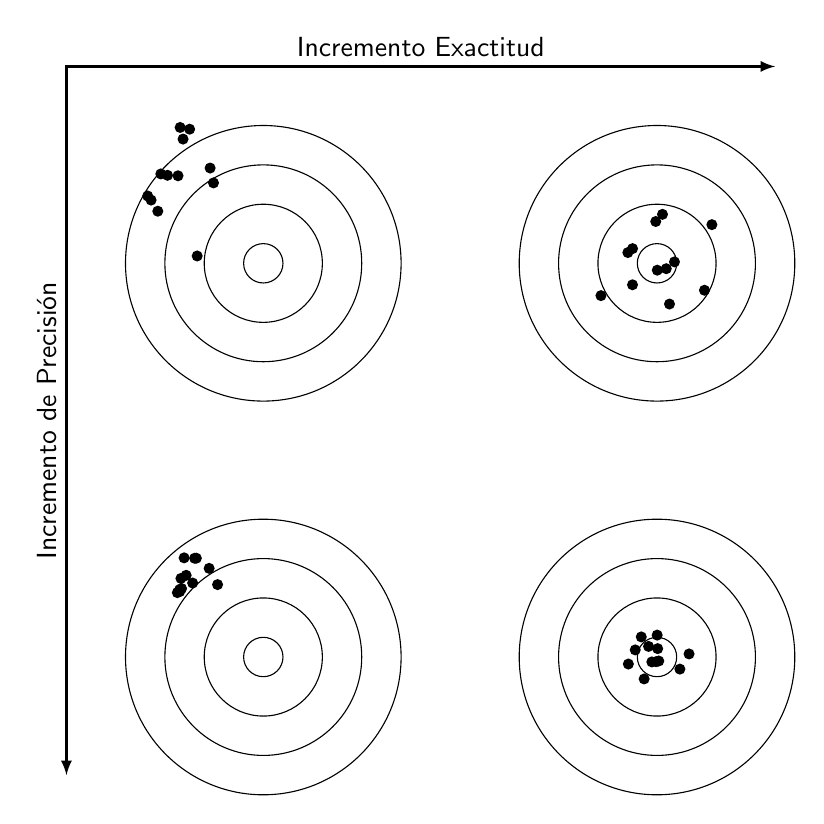
\begin{tikzpicture}[font=\sffamily]
\draw[latex-latex,thick](0,-9) -- node[midway,sloped,above] {Incremento de Precisión}
(0,0) -- node[midway,sloped,above] {Incremento Exactitud} (9,0);
%
\begin{scope}[shift={(2.5,-2.5)}]
 \foreach \X in {0.25,0.75,1.25,1.75}
 {\draw (0,0) circle (\X);}
 \foreach \X in {1,...,12}
  \fill (-1,1) + (rand*360:rand*1) circle(2pt);
\end{scope}
%
\begin{scope}[shift={(7.5,-2.5)}]
 \foreach \X in {0.25,0.75,1.25,1.75}
 {\draw (0,0) circle (\X);}
 \foreach \X in {1,...,12}
  \fill  (rand*360:rand*1) circle(2pt);
\end{scope}
%
\begin{scope}[shift={(2.5,-7.5)}]
 \foreach \X in {0.25,0.75,1.25,1.75}
 {\draw (0,0) circle (\X);}
 \foreach \X in {1,...,12}
  \fill (-1,1) + (rand*360:rand*0.5) circle(2pt);
\end{scope}
%
\begin{scope}[shift={(7.5,-7.5)}]
 \foreach \X in {0.25,0.75,1.25,1.75}
 {\draw (0,0) circle (\X);}
 \foreach \X in {1,...,12}
  \fill  (rand*360:rand*0.5) circle(2pt);
\end{scope}
\end{tikzpicture}
\end{document}
\caption{Relación entre Exactitud y Precisión.}
\end{figure}

\section{Definición de Error}
\subsection{Error Verdadero $(E_v)$}
Es la diferencia simple entre el valor Verdadero $(V_v)$ y el Valor Aproximado $(V_a)$:
$$E_v=V_v - V_a$$
Esta definición de error no toma en consideración la magnitud del valor que se está evaluando.
\subsection{Error Relativo Verdaderos}
Para introducir la magnitud del valor que ese está midiendo se normaliza el error $(E_r)$ al valor verdadero $V_v$:
$$E_r = \dfrac{E_v}{V_v}\cdot 100\% = \dfrac{V_v-V_a}{V_v}\cdot 100\% $$
En aplicaciones reales el valor verdadero $(V_v)$ únicamente se conocerá cuando se trate de funciones que tienen solución analítica. En general, el valor verdadero no se lo conoce. Se utiliza para ello la mejor estimación posible.
\\${ }$\\
Los métodos numéricos que utilizan sistemas iterativos, el error se normaliza, respecto de los valores aproximados. De esta manera, el error relativo aproximado se calcula por:
$$E_a = \dfrac{V_{actual}-V_{anterior}}{V_{actual}}\cdot 100\% $$
donde el $V_{actual}$ representa el último valor calculado y $V_{anterior}$ es el valor anterior en dos iteraciones sucesivas.
\\${ }$\\
El signo del error en general, no es significativo, siendo de mayor importancia acotar el valor absoluto del error $|E_a|$ menor a una cierta tolerancia. $E_s$, que en términos de la cantidad $n$ de cifras significativas utilizadas en el cálculo del error es:
$$E_s =0.5 \cdot 10^{2-n} \%$$
Donde:
\begin{itemize}
\item $n:$ Número de Cifras Significativas
\end{itemize}
Esta formula garantiza que el valor calculado tendrá $n$ cifras significativas iguales al valor verdadero.
\section{Series}
Las series son sucesiones de términos (en general infinitos) que se utilizan para representar funciones. El uso de series facilita el tratamiento de aquellas expresiones que son muy complicadas.
\subsubsection{Serie de Taylor}
$$f(x)=\displaystyle\sum_{n=0}^{\infty} \dfrac{ f^{(n)}(a) \cdot (x-a)^n}{n!} $$
Donde:
\begin{itemize}
\item $f^{(n)}(a):$ Derivada $n$-ésima de $f(x)$ evaluada en $a$.
\item $n!:$ Factorial de $n$.
\item $a:$ Entorno reducido de $x$.
\end{itemize}
\subsubsection{Serie de MacLaurin}
Es un caso particular de la serie de Taylor para $a=0$.
$$f(x)=\displaystyle\sum_{n=0}^{\infty} \dfrac{ f^{(n)}(0) \cdot (x)^n}{n!} $$
\section{Reglas de Redondeo}
\begin{enumerate}
\item En el redondeo se conservan las cifras significativas ,y el resto se descarta. El último dígito que se conserva se aumenta en una si el primer dígito descartado \textit{es mayor de 5}. De otra manera se deja igual. Si el primer dígito descartado \textit{es 5} o es \textit{5 seguido de ceros}, entonces el último dígito retenido se incrementa en uno solo si es impar.
\item En la suma y en la resta, el redondeo se lleva a cabo de forma tal que el último dígito retenido en la respuesta corresponda con el último dígito mas significativo de los números que se están sumando o restando.\\ Observar que un dígito en la columna de las centésimas es mas significativo que un número en la columna de las milésimas.
\item Para la multiplicación y para la división el redondeo es tal que la cantidad de cifras significativas del resultado es igual al número mas pequeño de cifras significativas que contiene la cantidad de la operación.
\item Para combinaciones de operaciones aritméticas, existen dos cosas generales. Se puede sumar o restar el resultado de las multiplicaciones o de las divisiones.
$$\binom{\textrm{Multiplicación o}}{\textrm{División}}\pm \binom{\textrm{Multiplicación o}}{\textrm{División}}$$
o también se pueden multiplicar o dividir los resultados de las sumas y restas.
$$\binom{\textrm{Suma o}}{\textrm{Resta}} \times / \div \binom{\textrm{Suma o}}{\textrm{Resta}}$$
en ambos casos se ejecutan las operaciones entre paréntesis y el resultado es redondeado antes de proceder con otra operación.
\end{enumerate}